\documentclass{article}
\usepackage[utf8]{inputenc}
\usepackage[spanish]{babel}
\usepackage{listings}
\usepackage{graphicx}
\usepackage{geometry}
\graphicspath{ {images/} }
\usepackage{cite}

\geometry{
textheight=23cm}
\begin{document}

\begin{titlepage}
    \begin{center}
        \vspace*{1cm}
            
        \Huge
        \textbf{INFORMA2 S.A.S}
            
        \vspace{0.5cm}
        \LARGE
        Parcial 2: Implementación
            
        \vspace{5cm}
            
        \textbf{Juan Pablo Cruz Gómez}
        
        \vspace{0.5cm}
        
        \textbf{Erika Dayana León Quiroga}
            
        \vfill
            
        \vspace{0.8cm}
            
        \Large
        Despartamento de Ingeniería Electrónica y Telecomunicaciones\\
        Universidad de Antioquia\\
        Medellín\\
        Septiembre de 2021
            
    \end{center}
\end{titlepage}

\tableofcontents
\newpage
\section{Sección introductoria}\label{intro}
En este informe se mostrará y explicará la implementación del problema presentado en el Parcial 2 de la materia Informática II, también se mostrarán las clases implementadas, los módulos del código implementado, la estructura del circuito montado en Tinkercad para la demostración del programa y los problemas que se presentaron durante el desarrollo de la implementación del problema.

\section{Clases implementadas} \label{clases}
En esta sección se presentarán las clases que se utilizarán para la solución del problema planteado.

\subsection{Clase QImage.}
Esta clase es proporcionada por Qt, sirve para el manejo de datos de imágenes, especialmente para el acceso y manipulación de pixeles. En este caso se utilizan los métodos que nos permiten conocer el número de pixeles a lo ancho y a lo largo de la imagen (.width, .height), para de esta forma obtener su tamaño. También se utiliza el método .pixelColor el cual retorna el color del pixel en unas coordenadas determinadas, en el caso de este problema se utiliza el .pixelColor dentro de un doble ciclo for que nos proporciona cada una de las coordenadas de la imagen, y de esta forma obtenemos la intensidad de color en cada uno de los pixeles de la imagen.



\section{Módulos del código implementado} \label{Modulos}
\begin{enumerate}
\item Se incluye el código para que el usuario ingrese la ruta del archivo por consola y de esta forma cargar la imagen que se encuentra en la misma con ayuda de la clase QImage. También se crea el archivo de escritura que se usará más adelante para sacar la información del procesamiento de la imagen.
Se declara el valor del alto y ancho de la imagen cargada anteriormente y el alto y el ancho de la matriz auxiliar que se usará para convertir la matriz original en una de 16x16.

\begin{figure}[h]
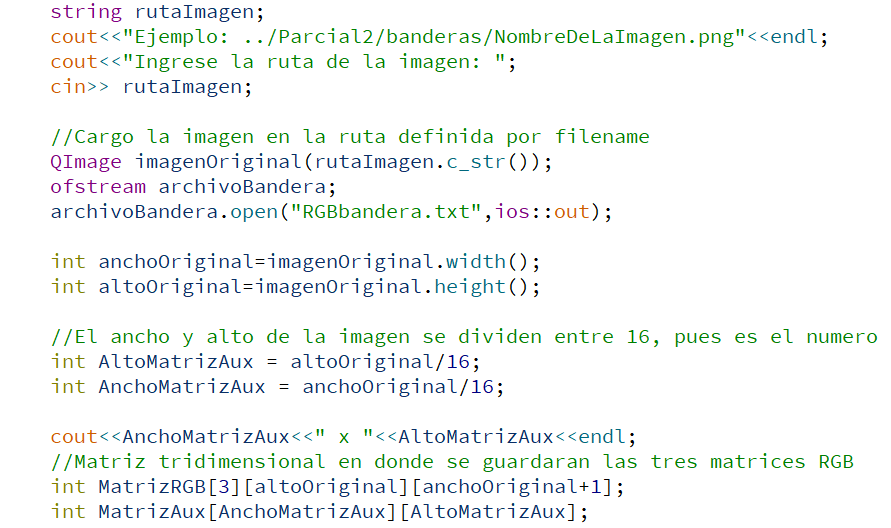
\includegraphics[width=10cm]{declaaracion.png}
\centering
\caption{Declaración de algunas variables}
\label{fig:declaracion}
\end{figure}


\item En esta parte del código se leen cada uno de los pixeles de la imagen para guardar su intensidad de color rojo, verde y azul, se hace uso de una matriz tridimensional llamada MatrizRGB para este propósito.

\begin{figure}[h]
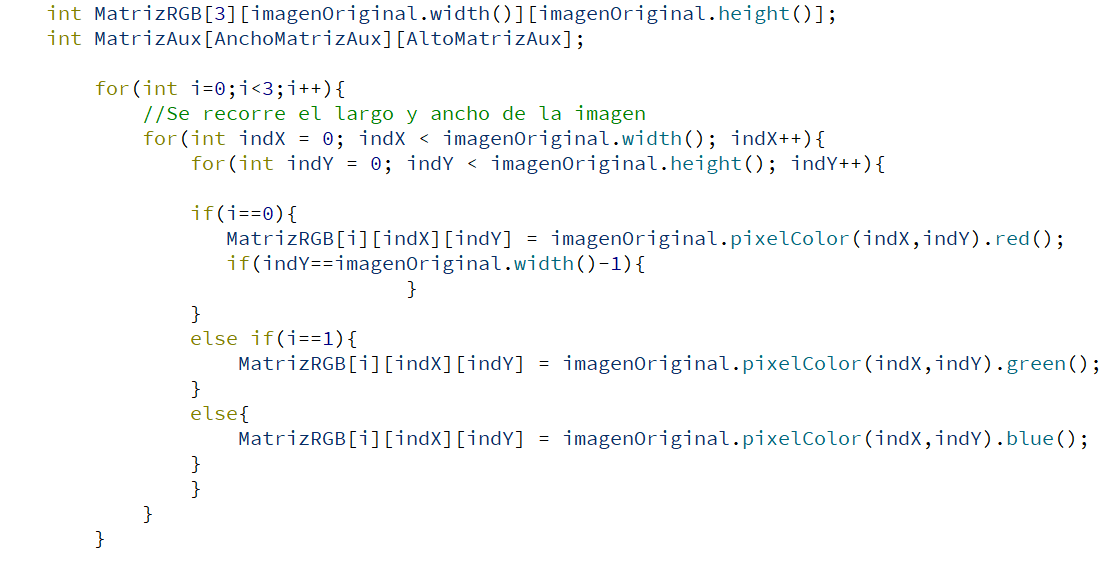
\includegraphics[width=15cm]{moduloMatrizRGB.png}
\centering
\caption{Matriz RGB}
\label{fig:matrizRGB}
\end{figure}

\item Después de tener las matrices de intensidad rojo, verde y azul guardadas en la metriz tridimensional MatrizRGB, procedemos a hacer el submuestreo de cada una de ellas, esto se logrará utilizando un while y un contador que se ocuparán de pasar por las tres matrices. Luego, a cada una de ellas se le irán sacando unas matrices auxiliares, las cuales tendrán un ancho y un largo de el largo y el ancho de las matrices originales dividido entre 16, que es el número de LEDs disponibles para la representación en Tinkercad.

\begin{figure}[h]
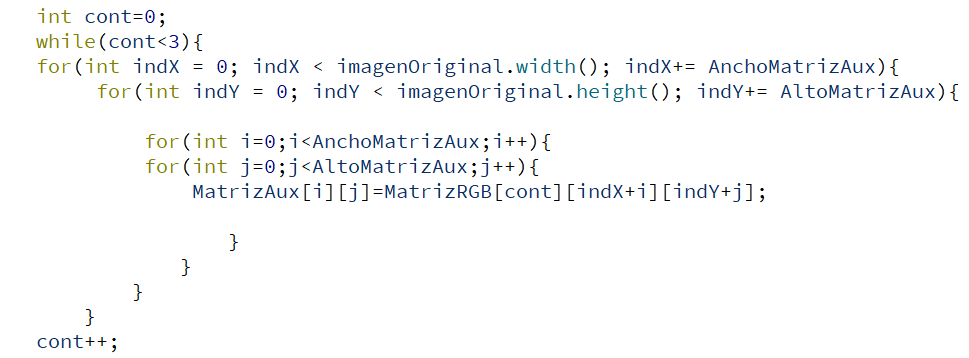
\includegraphics[width=15cm]{matrizaux.png}
\centering
\caption{Matriz auxiliar.}
\label{fig:matrizaux}
\end{figure}

\item Cada que se añade un elemento a la matriz auxiliar, este mismo elemento va sumándose con los demás elementos de la misma matriz para luego sacarle el promedio dividiendo entre la multiplicación del ancho por el alto de la matriz auxiliar. Este promedio calculado se va guardando en un arreglo llamado 'promedios' de tamaño 256.

\newpage
\begin{figure}[h]
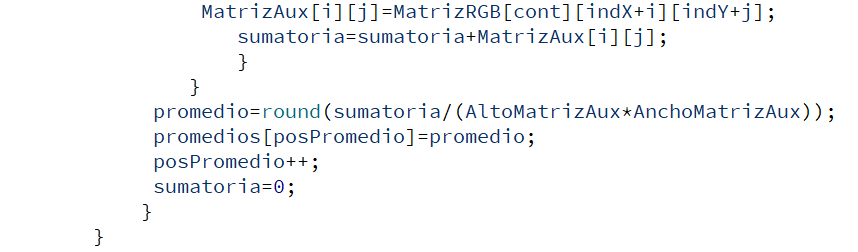
\includegraphics[width=15cm]{promedio.png}
\centering
\caption{Cálculo del promedio.}
\label{fig:promedio}
\end{figure}

\item Se recorre newMATRIZ que es la matriz obtenida por medio de promedios de la matriz original para convertirla a tamaño de 16x16, y se va rellenando haciendo uso del arreglo 'promedios', que iniciará en cero e irá aumentando de uno en uno hasta acabar el arreglo de tamaño 256.

En esta misma parte del código se escribe el archivo de texto llamado 'RGBbandera.txt', el cual contendrá la información de las tres matrices de intensidad necesarias para la simulación de Tinkercad.

\begin{figure}[h]
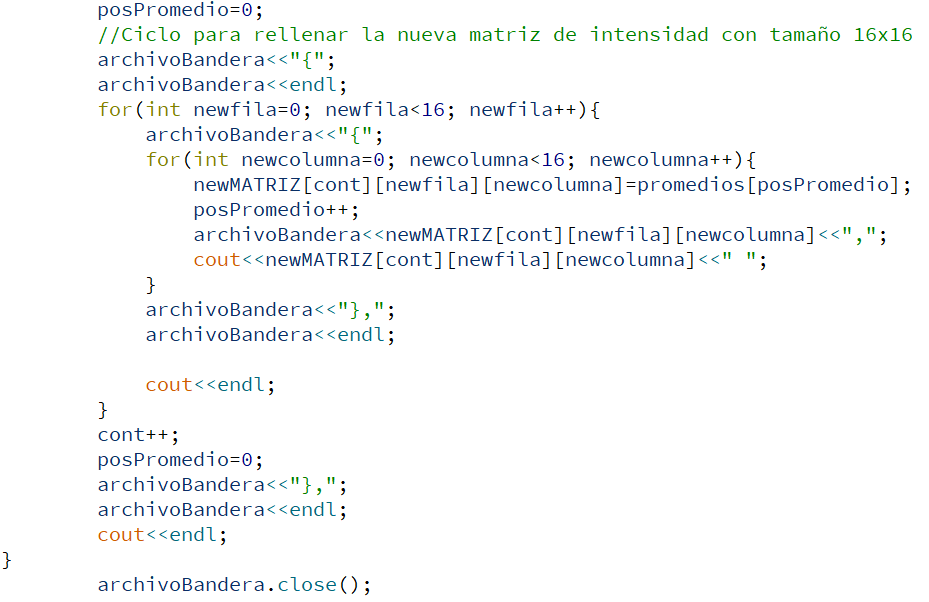
\includegraphics[width=13cm]{newmatriz.png}
\centering
\caption{Nueva matriz 16x16}
\label{fig:nuevamatriz}
\end{figure}

\end{enumerate}

\newpage
\section{Estructura del circuito} \label{circuito}

\begin{figure}[h]
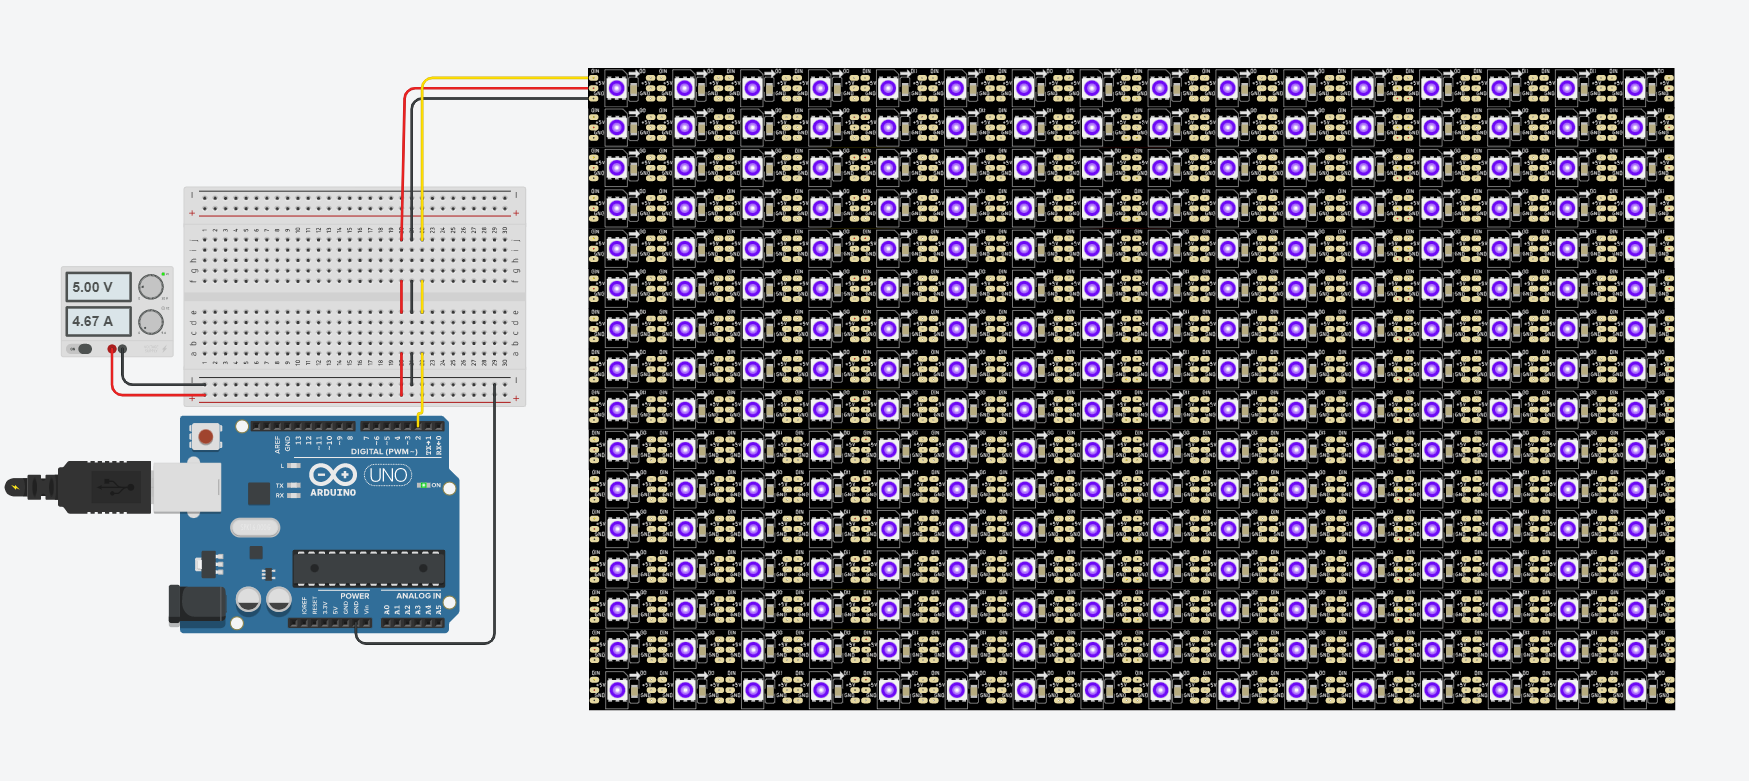
\includegraphics[width=15cm]{LEDs16x16.png}
\centering
\caption{Montaje de la matriz de LEDs de 16x16}
\label{fig:montaje}
\end{figure}


\section{Problemas presentados} \label{problemas}
El principal problema presentado fue el encontrar una forma de reducir o amplificar el tamaño de las imágenes a 16x16, que es el tamaño decidido para representar las imágenes mediante las tiras de Neo Pixeles.

No se hacía un submuestreo correcto ya que estábamos tomando en el código los componentes RGB de la imagen columna por columna y los estábamos guardando fila por fila, por lo cual no quedaban matrices con los componentes RGB correctas para se simulados en la plataforma de Tinkercad.


Teníamos problemas en la lectura de la matriz 16 x16 en tinkercad y se solucionó poniendo la matriz 16 x 17.

\section{Manual de usuario} \label{manual}
Siga los siguientes pasos para un correcto funcionamiento del programa.
\begin{enumerate}
    \item Ubique la carpeta en su computador en donde se guarda el programa de qt.
    
\begin{figure}[h]
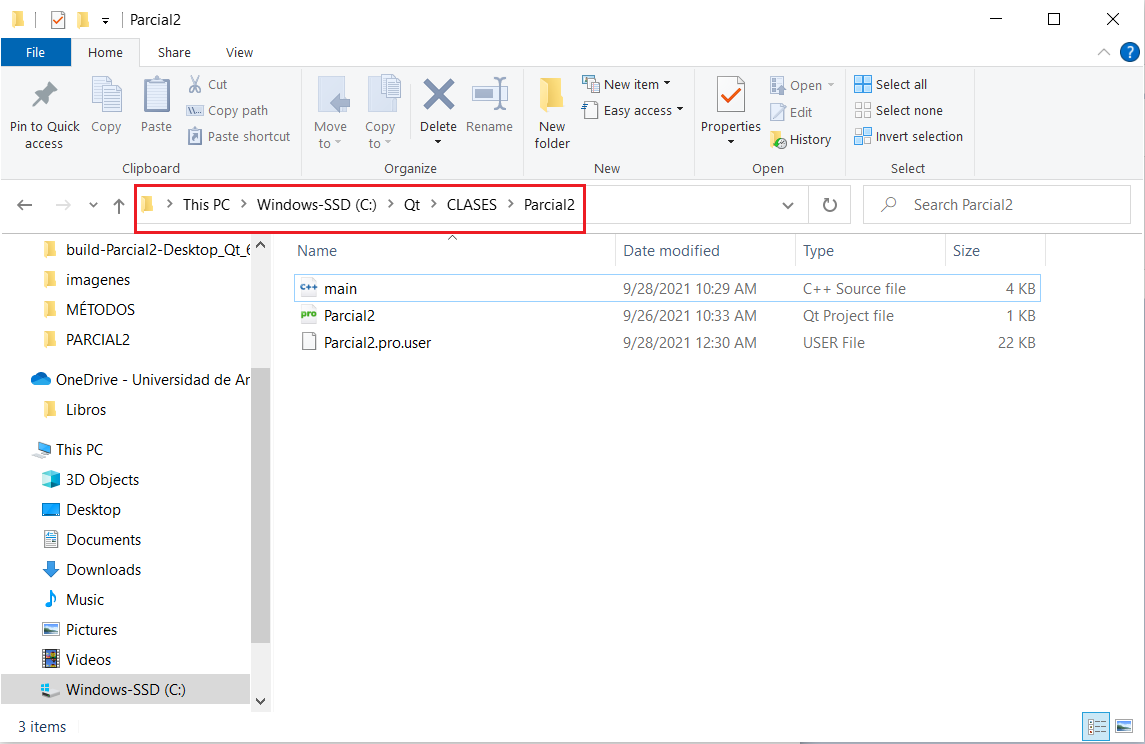
\includegraphics[width=12cm]{carpeta.png}
\centering
\caption{Ubicar la carpeta en donde se guarda el programa}
\label{fig:carpeta}
\end{figure}

\newpage

    \item Cree una carpeta para guardar en ella las imágenes de las banderas que posteriormente se procesarán.
\begin{figure}[h]
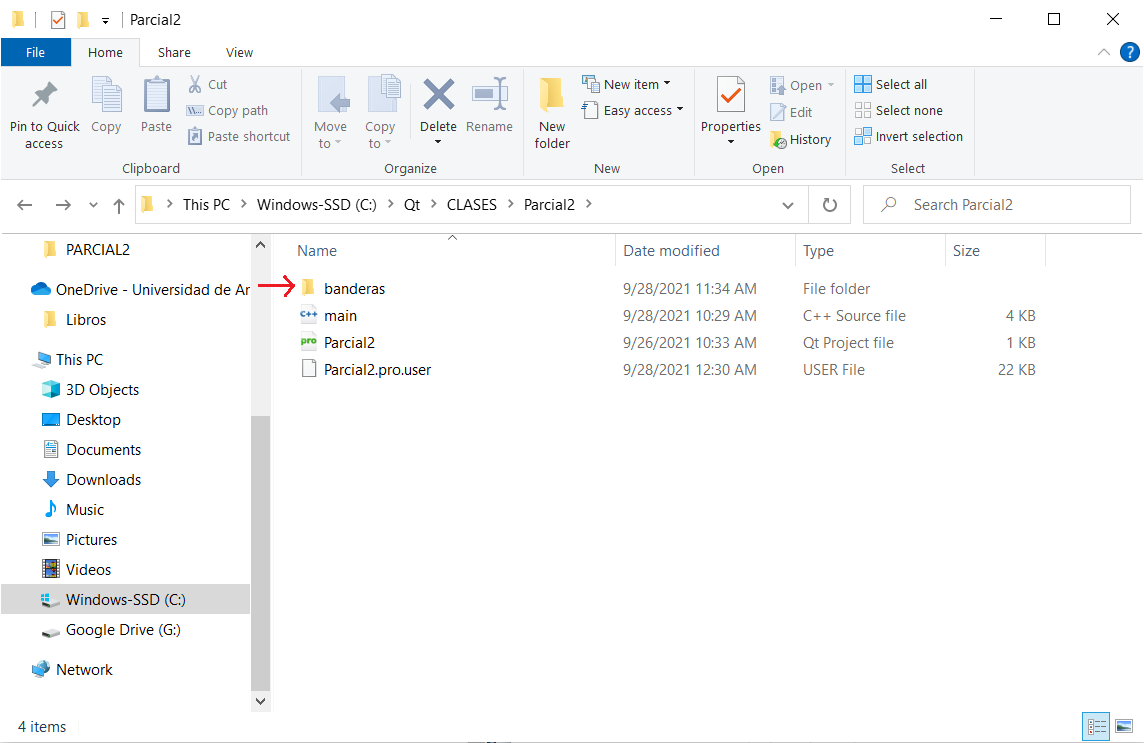
\includegraphics[width=12cm]{carpetabanderas.png}
\centering
\caption{Crear la carpeta en donde se guardarán las imágenes}
\label{fig:carpetabanderas}
\end{figure}
    
    \item Abra el programa y presione el botón ubicado en la parte inferior izquierda de su pantalla encerrado y señalado en rojo que se muestra en la figura \ref{fig:run} para iniciar el programa, o la combinación de teclas Ctrl+R.

\begin{figure}[h]
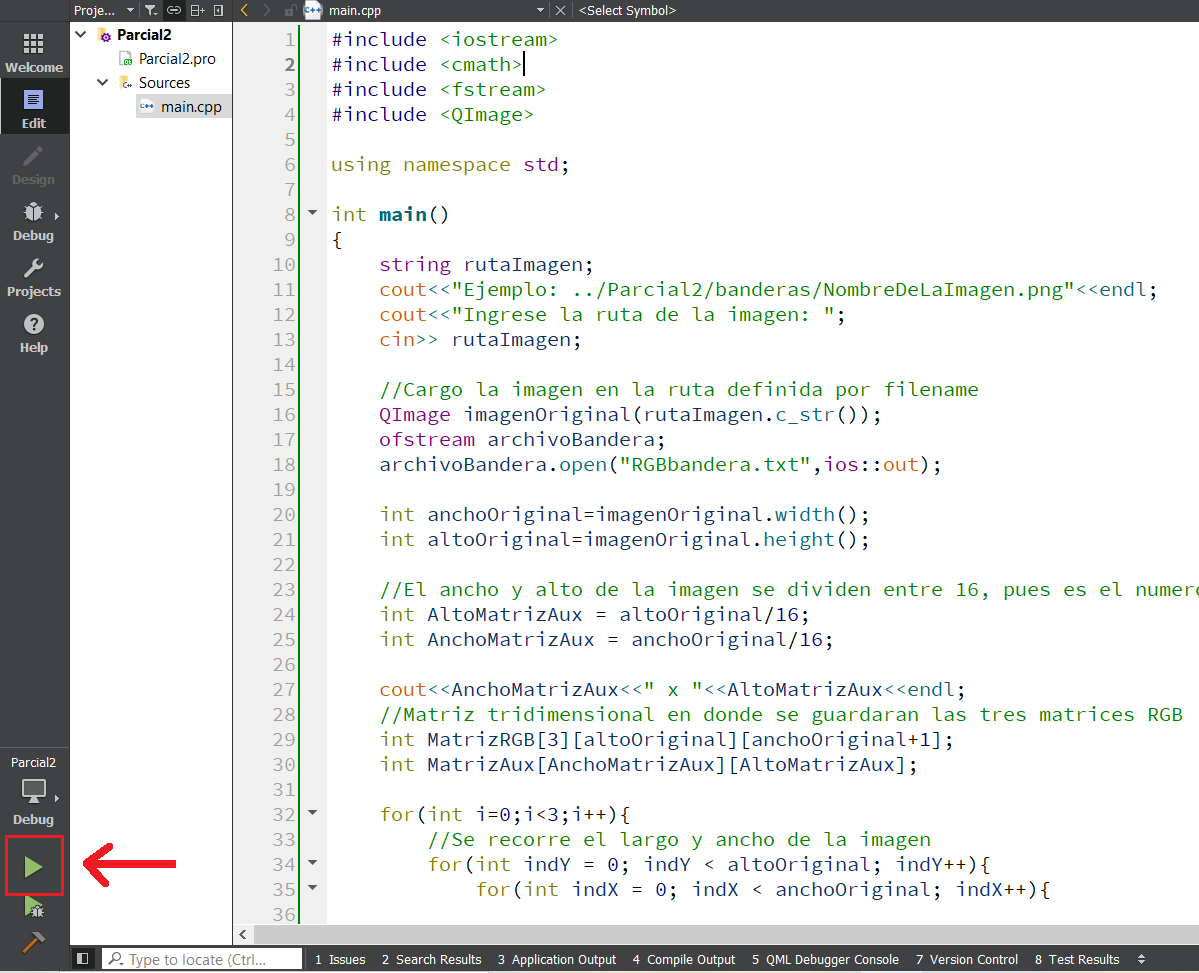
\includegraphics[width=7cm]{run.png}
\centering
\caption{Manual de usuario: Primer paso.}
\label{fig:run}
\end{figure}

\newpage
    \item Después de realizar el paso anterior, una ventana emergente como la que se muestra en la figura \ref{fig:paso2} se mostrará en la pantalla y será el lugar en donde se ingrese el único dato necesario para el programa. 
    El dato a ingresar es la ruta de la imagen y se muestra un ejemplo de cómo debe ser escrito.
    
\begin{figure}[h]
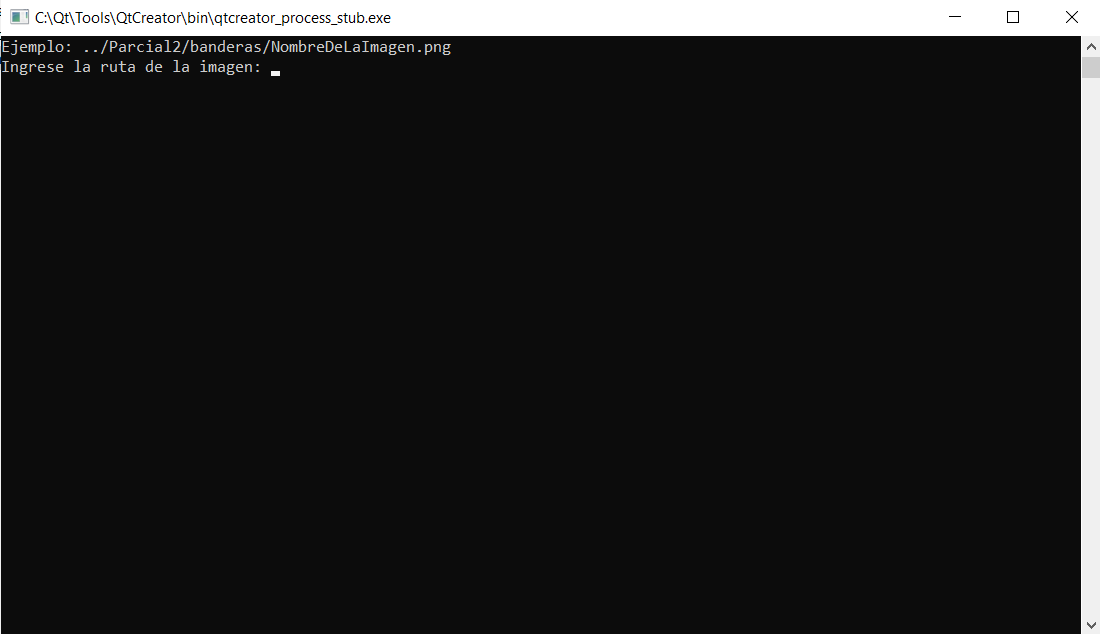
\includegraphics[width=15cm]{paso2.png}
\centering
\caption{Ingreso de datos.}
\label{fig:paso2}
\end{figure}

\begin{figure}[h]
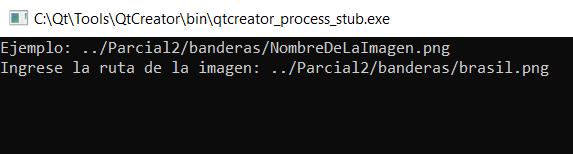
\includegraphics[width=15cm]{ejempaso2.png}
\centering
\caption{Ejemplo de ingreso de datos.}
\label{fig:ejempaso2}
\end{figure}

\newpage
\item Después de ingresar la ruta de la imagen el programa procesará la imagen y creará un archivo de texto en donde se guardará la información que se tiene que incluir en el código de Tinkercad.

El archivo de texto se guardará en una carpeta en la que su nombre comienza con 'build-' y sigue con el nombre de la carpeta en donde se guarda el programa, en este ejemplo 'Parcial2'.

\begin{figure}[h]
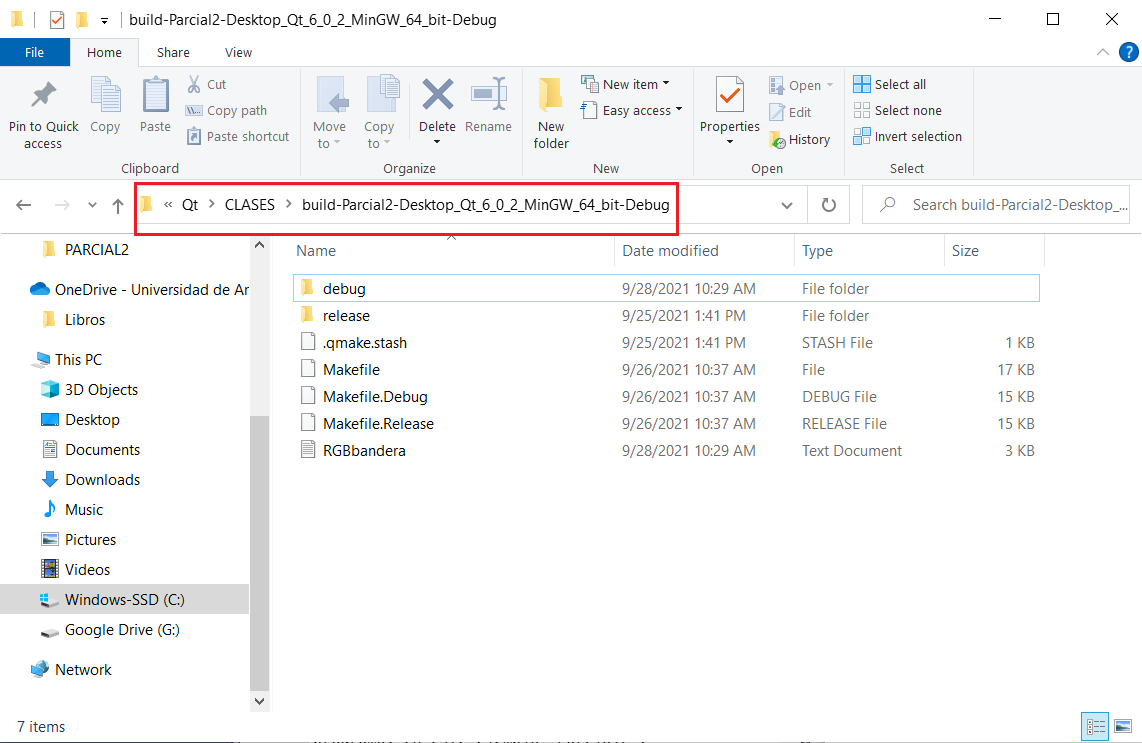
\includegraphics[width=15cm]{txt.png}
\centering
\caption{Ejemplo de ingreso de datos.}
\label{fig:txt}
\end{figure}
 \newpage
\item Se abre el archivo RGBbandera.txt y se copia todo su contenido.

\begin{figure}[h]
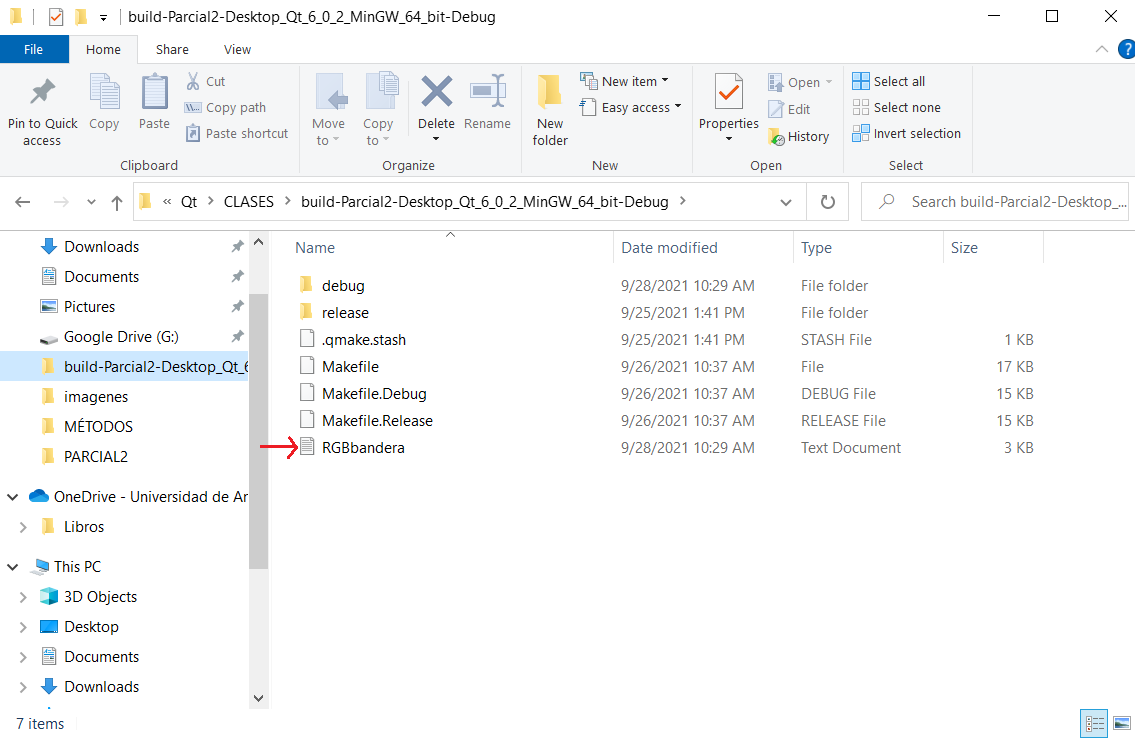
\includegraphics[width=10cm]{txtabierto.png}
\centering
\caption{Archivo .txt para abrir.}
\label{fig:txtabierto}
\end{figure}

\item Se abre en el navegador el siguiente link que nos llevará al circuito montado en Tinkercad: https://www.tinkercad.com/things/bFvlFZ9hjM0

Posterior a esto se abre la ventana de código y en la sección demarcada con '//COPIAR TEXTO DESDE  ESTE PUNTO' se copia el contenido del archivo RGBbanderas.txt.

\begin{figure}[h]
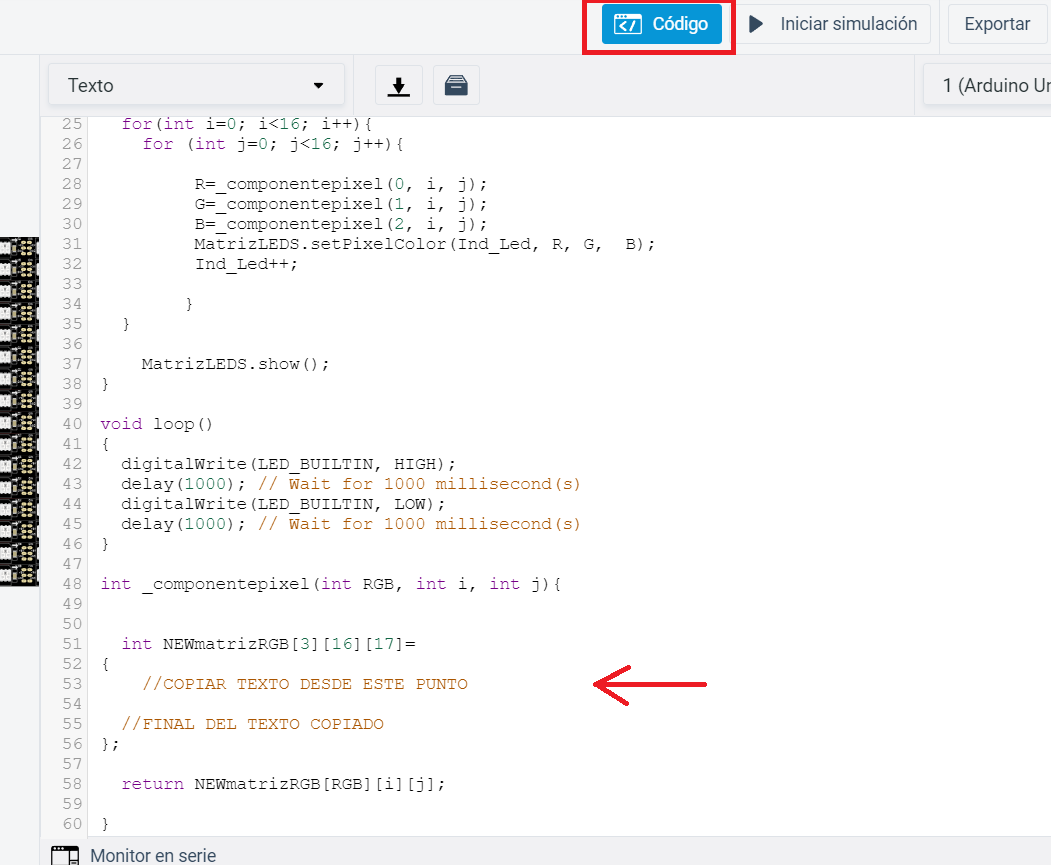
\includegraphics[width=10cm]{tinkercad.png}
\centering
\caption{Tinkercad.}
\label{fig:tinkercad}
\end{figure}

\begin{figure}[h]
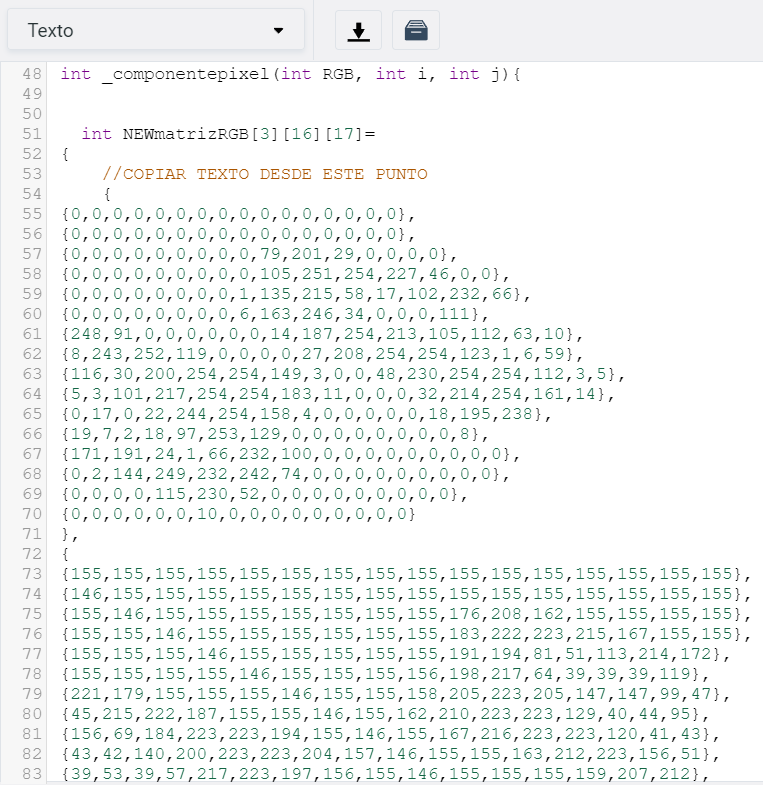
\includegraphics[width=10cm]{ejemtinkercad.png}
\centering
\caption{Ejemplo de la información copiada del archivo.}
\label{fig:ejemtinkercad}
\end{figure}

\begin{figure}[h]
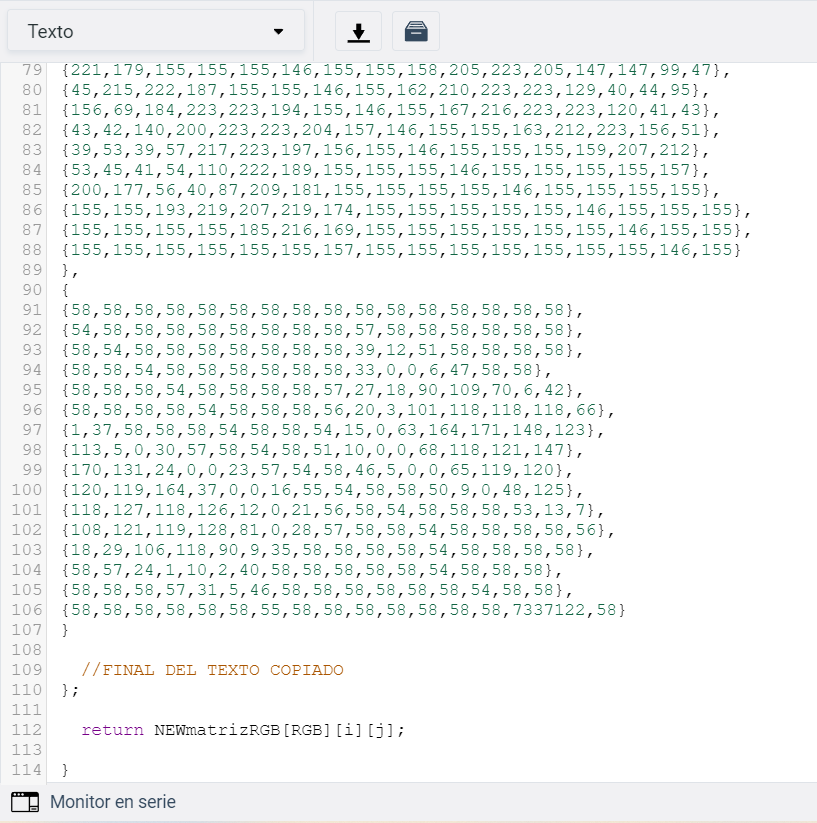
\includegraphics[width=10cm]{ejem2.png}
\centering
\caption{Ejemplo de la información copiada del archivo.}
\label{fig:ejem2}
\end{figure}


\end{enumerate}
\end{document}
